
%(BEGIN_QUESTION)
% Copyright 2013, Tony R. Kuphaldt, released under the Creative Commons Attribution License (v 1.0)
% This means you may do almost anything with this work of mine, so long as you give me proper credit

A tank holding 13 feet of liquid exerts an hydrostatic pressure on the gauge mounted at the bottom:

$$\includegraphics[width=15.5cm]{i02822x01.eps}$$

Calculate the magnitude of this hydrostatic pressure, in units of PSI:

\vskip 10pt

$P$ = \underbar{\hskip 50pt} PSI

\vskip 10pt

\underbar{file i02822}
%(END_QUESTION)





%(BEGIN_ANSWER)

$P$ = \underbar{\bf 4.324} PSI
 
%(END_ANSWER)





%(BEGIN_NOTES)


%INDEX% Physics, static fluids: hydrostatic pressure

%(END_NOTES)


